
\section{The Mixed Weighted Straight Skeleton}
\label{sec:mwss}

% Do we want to say that the PWSS may not grow (if all theta zero),?

% todo: we had this for pwss, how can we work it in here? We note that in all situations, the region collapsing at any time is locally topologically equivalent to a disc immediately before the event. The disc may be bounded on some sides, and unbounded on others.  When this is the case, the collapsing area is again locally equivalent to the topological disc.

The final variation of the SS we will introduce is the \emph{mixed weighted straight skeleton} (MWSS). This structure allows the angle of the direction planes, $\theta$, to be positive and negative over edges in a single plan. As before we introduce some of the issues surrounding degeneracies, and present a partial algorithm for resolving them.

%: $-\frac{\pi}{2} < \theta < \frac{\pi}{2}$. Inititively this allows the edges of the active plan to move towards the interior or exterior at the same time.
As in the PWSS case, $\theta$ is limited to avoid infinitely fast edges on the active plan, allowing only  $-\frac{\pi}{2} < \theta < \frac{\pi}{2}$. Therefore a $\theta < 0$ implies that an active plan edge is moving away from the interior of the polygon, a $\theta = 0$ implies an edge that does not move, and a $\theta > 0$ implies an edge moving towards to interior of the polygon. 
%The angle defines the slope of the face associated with that edge of the input plan. That is, $\theta$ defines the speed of the edge on the active plan as the sweep plan rises.

The MWSS enables more 3D terrains to be defined; The set of skeletons definable are a superset of the SS, PWSS and NWSS schemes. For example the active plan can grow, as well as shrink, or can be a mixture of both. Therefore certain MWSSs may not terminate after the final event, the enclosed area may continue growing indefinitely as the sweep plane rises. It is an open problem to determine if a given MWSS will terminate if it contains any values of $\theta < 0$, without executing the skeleton calculation itself. Fig.~\ref{fig:wss_unbounded} gives an example in which the resolution of a borderline case differentiates between an non-terminating skeleton, and a terminating one.

\begin{figure}
  \centering
  \def\svgwidth{1.0\columnwidth}
  \includesvg{12-skeleton/images/wss_unbounded}
  \caption[Unbounded MWSS]{\label{fig:wss_unbounded}MWSS that are bounded (left) and unbounded (right). The red face grows to an infinite area as the sweep plane rises. A small peturbation to the input plans is the only difference between these PWSS, which is sufficient to change the edge emerging from the orange intersection. }
\end{figure}

Given the additional degrees of freedom available in the MWSS we expect that to encounter the degenerate cases observed in the SS and PWSS cases. In addition there are are a new class of \emph{point degeneracies} observable.

\subsection{Point degeneracies}

% this is the +-WSS degeneracy section.
%As shown in Fig.~\ref{fig:Impossible} there are events where common sense does not easily give an solution to.

If all the edges are moving inwards or outwards, as with the PWSS or NWSS, the SS GIE introduced in Sec.~\ref{s:gie} is still suitable. However there is a complex set of degenerate events that may occur with some angles of $\theta > 0$ and some $\theta < 0$. An example is given in Fig.~\ref{fig:wss_strange}.

\begin{figure}
  \centering
  \def\svgwidth{1.0\columnwidth}
  \includesvg{12-skeleton/images/wss_strange}
  \caption[Degenerate events in the PWSS and MWSS]{\label{fig:wss_strange}. Left: A complex event in a PWSS, over a plan (green). Right: A MWSS in which four areas merge to become one. Note that the 3D models are the resulting meshes of a skeleton as some MWS Skeletons are difficult to illustrate in 2D. }
\end{figure}


A more complex example of a simple eventFig.~\ref{fig:wss_example_topology}, which shows a possible event with many edges colliding. Here we can see chains of edges representing bounded, as well as unbounded areas, loops, and \emph{enclosed chains} (Fig.~\ref{fig:wss_enclosing_chain}), all colliding at one point. Fig.~\ref{fig:wss_union_vs_gie} gives an example of the GIE failing to process an event. Indeed every edge of an arbitrary polygon may be coerced to collide at any point by altering the per edge values of $\theta$.

\begin{figure}
  \centering
  \def\svgwidth{1.0\columnwidth}
  \includesvg{12-skeleton/images/wss_example_topology}
  \caption[A point degeneracy]{\label{fig:wss_example_topology} Left: The active plan just before an event. A complex set of chains collide at a single event (orange). Right: after the intra-chain step and one-chain step of the GIE the topology is simplified. Note that the curved edges marked with an asterisk represent the topology of two colinear straight edges.}
\end{figure}

\begin{figure}
  \centering
  \def\svgwidth{0.4\columnwidth}
  \includesvg{12-skeleton/images/wss_enclosing_chain}
  \caption[Enclosing chains]{\label{fig:wss_enclosing_chain} We describe the chain \emph{a} as enclosing chain \emph{b}, as $\phi < \pi$. The chains are shown here before a collision at the orange point.}
\end{figure}

We wish to have a consistent solution to these degenerate events, such as those at the bottom of Fig.~\ref{fig:wss_options}. That is, the plan remains well formed after the event. 

We have been unable to find a elegant general solution to the problem!

Here we present an engineered solution that is as consistent as possible with the existing definition of the unweighted skeleton. Other characteristics that are desirable in a solution for such events include:
\begin{itemize}
\item{Similarity to the SS.}
\item{Consistency with the SS when all angles are a positive constant.}
\item{Consistency with the PWSS when all angles are positive.}
\item{Invariance to rotation of the plan. As with the the straight skeleton the result of an event should not depend on the orientation of the plan.}
\end{itemize}
 
\begin{figure}
  \centering
  \def\svgwidth{1.0\columnwidth}
  \includesvg{12-skeleton/images/wss_options}
  \caption[Several solutions to the MWSS]{\label{fig:wss_options}Above: Four chains collide at an event (orange point). The desired plan topology after the event is unclear. We must keep the input edges (red) in the same locations to remain consistent with the remainder of the plan. Below: There are many possible options for the topology change at the event. (Note that we show the active plan a time after the event.) Some use existing edges, others create new edges (initially these new edges are zero length, but subsequently grow) during the event.}
\end{figure}

In order to provide a suitable resolution to these events we simplify the edges by first removing zero length edges, and then removing zero area chains.

To simplify the active plan situation we can apply the SS intra chain step and one chain step, Fig.~\ref{fig:wss_example_topology} right, to remove edges that shrink to zero length. The intra chain step also removes loops of edges involved in the event; As they approach an event they shrink to zero length and area, and as such we may remove them from the active plan, and not consider them further in the event handling.

\subsection{Parallel Edges}



\begin{figure}
  \centering
  \def\svgwidth{1.0\columnwidth}
  \includesvg{12-skeleton/images/skel_impossible}
  \caption[A MWSS event with four parallel edges]{\label{fig:skel_impossible}.}
\end{figure}


%We now define several features of the MWSS that help us. The major axis, approaching edges and the sector properties.

%The \emph{major axis} defines the direction that all chains of length one take. There may be more than one chain of length one in the MWSS, Fig.~\ref{fig:wss_example_topology}. However it is impossible for these chains to have more than one orientation in a single event as it occurs at a single point.

%\begin{figure}
%  \centering
%  \def\svgwidth{0.5\columnwidth}
%  \includesvg{12-skeleton/images/wss_major_axis}
%  \caption{\label{fig:wss_major_axis}At an event (orange) we may not have more than one orientation of chains of length one. %If this were the case (above), there would be a point (red) which the 1-chains (green and blue) arrived at before the event. There would, therefore, have been another (red) event which combines these edges before they arrive at the first event (orange).}
%\end{figure}

At an event all the edges involved in the collision approach the location at an angle defined by the edge's current orientation. Fig.~\ref{fig:wss_ordered_point}, left, shows the orientation-ordered points for Fig.~\ref{fig:wss_example_topology}. Any edges that do not approach according to their angle must have been removed by an earlier collision, Fig.~\ref{fig:wss_ordered_point}, right. This property is known as the \emph{$\ge$ approaching edges} property. This refers to the fact that the angle between consecutive edges around an intersection is equal to, or greater than, zero.

The situation that complicates further processing is approaching edges with the same angles. That is when two parallel edges, with different directions approach an event from the same side. The area between these edges approaches zero near the event, and should be removed by the loop of two rule. Therefore we remove these adjacent, parallel edges with the same orientation at the event, Fig.~\ref{fig:wss_equal_approach_killer}. After we remove these lines, we can say that the event has the \emph{$>$ approaching edges property} as all the angles between adjacent approaching edges are greater than zero.

\begin{figure}
  \centering
  \def\svgwidth{1.0\columnwidth}
  \includesvg{12-skeleton/images/wss_equal_approach_killer}
  \caption[Removing zero area chains]{\label{fig:wss_equal_approach_killer} After the intra-chain step we remove all the zero area chains, leaving the topology shown (top, left). We show the chains just before the event for clarity. The black lines connect (asterisked) edges which would become adjacent and parallel at the event. We convert these pairs of edges into single chains as shown. We either use the interior bias (top right) or exterior bias (bottom left). 
%todo, does this work without loop of two?: After the corresponding events at remote sites, we will remove these chains using the loops of two rule (bottom right).
}
\end{figure}

\begin{figure}
  \centering
  \def\svgwidth{1.0\columnwidth}
  \includesvg{12-skeleton/images/wss_linear_align}
  \caption[Global coordiation of a solution with parallel edges]{\label{fig:wss_linear_align} Given a plan (top left) that leads to a number of events (top middle, red blue and yellow circles) at the same height, which share a single edge (top middle, edge a), there are several possible solutions. We wish to avoid creating parallel, colinear edges that will immediately self-intersect again (top right), that is we must have a globally coordinated solution. Where there are an odd number of parallel edges approaching an intersection from the same direction we introduce two globally consistent options; Interior bias (bottom left) or exterior bias (bottom right).}
\end{figure}

To remove the edges, and keep the global-consistency property defined above, we must make a local choice that is globally consistent, Fig.~\ref{fig:wss_linear_align}. In a similar manner to the SS case, we connect these pairs of adjacent lines. At the other end of these parallel edges, another event at the same height must make consistent choices, such that we never have two coincident, overlapping, edges in the active plan, Fig.~\ref{fig:wss_linear_align} top right.

This situation presents another choice. More than two approaching edges can have the same angle, Fig~\ref{fig:wss_equal_approach_killer}. If there are an even number of such edges at one angle, the adjacent pairs of edges can be connected together. However if there are an odd number of edges, we have to choose which adjacent pairs to merge. Here we present two solutions:
\begin{itemize}
\item{\emph{interior bias:} The pairs of lines surrounding an interior region of the plan form a loop of two.}
\item{\emph{exterior bias:} The pairs of lines surrounding an exterior region of the plan form a loop of two.}
\end{itemize}

\begin{figure}
  \centering
  \def\svgwidth{1.0\columnwidth}
  \includesvg{12-skeleton/images/wss_ordered_point}
  \caption[Ordering chains around the event]{\label{fig:wss_ordered_point} As the chains of edges in the MWSS approach the event (orange) they become ordered (left). If this were not the case (right), they would have intersected during an separate earlier event (red).}
\end{figure}


\subsection{Other Observations}

include: multiple possible solutions
5 star constructive failures.

Another interesting fact can be observed by not handling an event, Fig.~\ref{fig:wss_sector}. If we ignore the rest of the plan away from the event, we may see that after the event the chains remain in the same configuration. More specifically the intersections of any edges remain at the same angle relative to the event location, Fig.~\ref{fig:skel_sector_2}, until another event may occur. We can see that this is true by recalling that the edges move in a direction parallel to themselves at a constant angle. They also all pass through the event location at the event at the same time. Therefore any intersections between these lines also move with constant speed directly away from the event location, that is they keep the same angle. We refer to this property as the \emph{sector property}.

The sector property can also be observed before an event, but after any preceding events. We can therefore view it as the trivial statement ``between events, no events occur''.

\begin{figure}
  \centering
  \def\svgwidth{1.0\columnwidth}
  \includesvg{12-skeleton/images/wss_sector}
  \caption[An example of the sector property]{\label{fig:wss_sector}The plan (green, blue and yellow areas) undergoes an event (orange). The sector property states that topology of the active plan corners remains unchanged immediately after the event (after 1, through after 2).}
\end{figure}

\begin{figure}
  \centering
  \def\svgwidth{0.5\columnwidth}
  \includesvg{12-skeleton/images/wss_sector_2}
  \caption[The sector property]{\label{fig:skel_sector_2}After an event (orange), any intersection between two edges, such as a corner, remains at constant angle, $\gamma$, relative to the event location. This gives rise to the sector property.}
\end{figure}

It is unclear how to handle the chains further. In all examples examined, there is always a solution that does not introduce any new (initially 0-length) edges into the active plan during the event, Fig.~\ref{fig:wss_hand_examples}. However it remains an open problem to consistently calculate this solution. While some sort of search technique may give the correct answer, we feel that there is may be a more elegant solution.

\begin{figure}
  \centering %LOST?!
  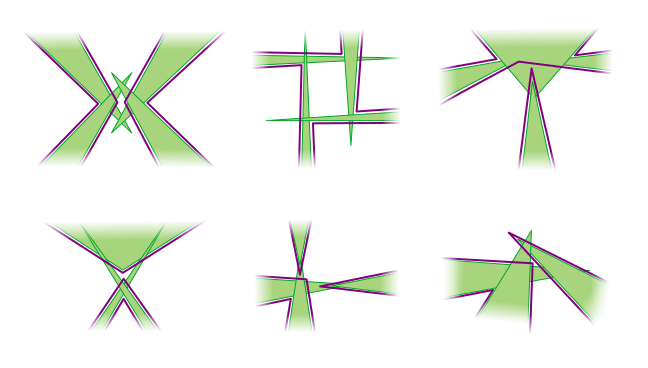
\includegraphics[width=1.0\columnwidth]{wss_hand_examples.png}
  \caption[Manual examples of good MWSS solutions]{\label{fig:wss_hand_examples} Several example events and solutions that do not require 0-length edges to be introduced into the active plan. The chains (green dashed lines) are shown after the event (orange). Certain good solutions are shown in purple, although there may be more than one solution for each situation.}
\end{figure}

\begin{figure}
  \centering
  \def\svgwidth{0.5\columnwidth}
  \includesvg{12-skeleton/images/wss_incremental}
  \caption[The sector property]{\label{fig:wss_incremental}FIXME.}
\end{figure}

\subsection{Multiple union approach}

This section presents an algorithm that does introduce zero length edges, the \emph{multiple union} approach. We analyse the topology immediately after an event, and perform area-unions with sets of edges to decide on an edge topology for after the event. Note that by the sector property, this topology of the chains is independent of time after the event. Therefore we define an ordering over the chains so that they can be added or subtracted from the \emph{output topology}. We use 2D Boolean geometry operations to build up this topology.

We start by ordering the chains into enclosed \emph{levels} of chains they contain before the event, Fig.~\ref{fig:wss_numbered_union}. The levels are enumerated from the location of the event, towards the deepest level. If the location (before the event) is inside (respectively outside) the region the output topology is initialised to be an inside (outside) region. Using the chains after the event, we iterate over the level, starting with the lowest-ordered level chains and add or subtract the union of all chains at that level them from the output topology as explained by Fig.~\ref{fig:wss_gie_example}. 

\begin{figure}
  \centering
  \def\svgwidth{1.0\columnwidth}
  \includesvg{12-skeleton/images/wss_numbered_union}
  \caption[Identify the level of chains]{\label{fig:wss_numbered_union} The levels of two different events. Note how the location of the event changes the definition of the levels. A chain's level is $1$ if it is adjacent to the event, otherwise it is one higher than the enclosing chain.}
\end{figure}

Because the angles between consecutive chains around a point is always greater that zero (by the \emph{$>$ approaching edges} property), we can be sure that the output topology will be compatible with the global active plan.

While this is one solution to this relatively rare problem, there are situations where the result isn't equivalent to the SS, and other quite strange topologies can occur, Fig.~\ref{fig:wss_union_vs_gie}

\begin{figure}
  \centering
  \def\svgwidth{1.0\columnwidth}
  \includesvg{12-skeleton/images/wss_union_vs_gie}
  \caption[A comparison of the GIE and multiple union procedure]{\label{fig:wss_union_vs_gie} In the MWSS, the GIE and the multiple union procedure  have different advantages. In the top example, the GIE creates the best output, without 0 length edges, while in the bottom example it creates an undesirable inverted (red) region on the now badly formed active plan. The multiple union procedure adds additional zero length edges in the first example, but always creates valid geometry (top and bottom examples). Compare to ``perfect'' manual results in Fig.~\ref{fig:wss_hand_examples}.}
\end{figure}

\begin{figure}
  \centering
  \def\svgwidth{1.0\columnwidth}
  \includesvg{12-skeleton/images/wss_gie_example}
  \caption[A multiple union calculation]{\label{fig:wss_gie_example} An example multiple union calculation. Given an input plan (a), several edges (marked with an asterisk) may collide (orange point). The edges involved can be split into levels, just before the event (b). After the event we can view the topology without intersections (d: green chains bound interior regions, white chains bound exterior regions). We can then use an union operation on those chains in the first level (e), before calculating the union of those chains in level 2 (f, yellow). We can then subtract the second level from the first (g). Because of the sector property, this new topology of edges will not intersect immediately after the event. It is also still compatible with the global geometry (h).}
\end{figure}

\FloatBarrier
\section{Summary}

This chapter has introduced four varieties of the straight skeleton - the unweighted straight skeleton, the positively weighted skeleton, the negatively weighted straight skeleton and the mixed weighted straight skeleton. Three of these skeletons form a chain of generalisation as the requirements on the angle of the direction planes are relaxed; SS $\subseteq$ PWSS $\subseteq$ MWSS. Each additional generalisation has brought with it additional degenerate cases that we have presented, and suggested solutions for. We have introduced a new general intersection event that gracefully handles the events encountered by the SS, PWSS and NWSS. Finally we introduced one flawed solution to the events encountered by the MWSS, and introduced an unproved theorem that a perfect solution always exists.



